\chapter{Implementation}
My implementation of the design presented before is a piece of
software written in C++ that depends on a few elements from GNU Radio,
gr-gsm and the official libhackrf C library~\cite{libhackrf}.\
libhackrf provides a configurable interface with the HackRF One and
that leaves a simple data structure to communicate with the
device. GNU Radio and gr-gsm brings signal processing software
implementations of things like low pass filters, frequency-
measurements and feedback information for frequency correction.

The project is hosted online and is located at
\url{https://github.com/martinjlowm/telecan}. The implementation uses
CMake~\cite{cmake} as its build- and project management system in
conjunction with Google Test~\cite{googletest} and Google
Mock~\cite{googlemock} C++ testing frameworks. The structure of the
project is as follows.
\begin{itemize}
\item \textbf{src/} --- The root of all the source code which further
  divides the code into multiple subdirectories. The directory ttself
  contains three source code files; the base analyzer,
  \textbf{base\_analyzer.cc}, some helper functions,
  \textbf{helper\_functions.cc} and the entry point,
  \textbf{telecom\_analyzer.cc}. The associated header files,
  \textbf{.h}, are located in the same directory which also applies
  for the following subdirectories.

  \begin{itemize}
  \item \textbf{device/} --- Source code for supported devices and
    their local data structures are placed here. The HackRF One
    interface and a circular buffer implementation reside in this
    directory.

  \item \textbf{dsp/} --- This directory holds digital signal
    processing source code and it, at the time of this writing, only
    has a refractional resampler implementation from the GNU Radio
    project.

  \item \textbf{gsm/} --- All \gls{GSM} related source code is placed
    in this directory and its subdirectory,
    \textbf{state\_machine}. It contains files similar to the blocks
    in \cref{fig:implementation_design}, in \cref{cha:design}, apart
    from a burst counter and a Viterbi detector. The Viterbi detector
    is a slightly modified version of the symbol sequence estimator of
    the same name found in gr-gsm~\cite{grgsm} by Piotr Krysik and is
    based on GSMsim~\cite{ekstr1997a}. The burst counter keeps track
    of the time synchronization feedback provided by the \gls{SCH}.

    \begin{itemize}
    \item \textbf{state\_machine/} --- The implementation consists of
      two \glspl{FSM}, a synchronization- and a \gls{FCCH} search
      state machine and they are both placed in this directory.
    \end{itemize}

  \item \textbf{umts/}: This directory is reserved for \gls{UMTS}
    specific code.

  \item \textbf{lte/}: Similar to \gls{UMTS}, this directory is
    reserved for an \gls{LTE} implementation.
  \end{itemize}

\item \textbf{lib/}: CMake is configured to look for Google Test and
  Google Mock in this directory, which must be downloaded and
  extracted manually if testing is desired. The directory is otherwise
  unused.

\item \textbf{test/}: A few unit tests for some of the source code
  reside in this directory.
\end{itemize}


This chapter introduces the data structures and methods that are used
in the implementation of the design to accomplish the functionality of
parsing \gls{GSM} mobile traffic on a specific channel. Similar to the
design chapter, this chapter also describes the implementation from
the bottom and up as the samples are processed.

\section{HackRF One interface}
The \gls{ADC} in the HackRF One, MAX5864, provides dual $8$-bit
\gls{I}/\gls{Q} samples which are transferred over the \gls{USB}
interface and written to a circular buffer. The transfer is configured
with a callback function that ensures samples to be locally
available. Upon filling the local circular buffer, these samples are
converted to a complex type with each term as a float data type. The
main loop of the application iterates this buffer to continuously
process the available samples and pass them along to the specified
analyzer. In this situation, with just one inheritor, the \gls{GSM}
analyzer is the receiver of these samples.

\section{GSM analyzer}
The \gls{GSM} analyzer inherits the properties of the base analyzer
and interfaces directly with the \gls{SDR} source. It acts upon
frequency feedback from the synchronization state machine and ensures
that samples are filtered by a low pass filter and downsampled from
two million samples per second to a multiple of the \gls{GSM} bit
rate, $270.83\si{kb/s}$. The analyzer is defined to use an
oversampling ratio of $4$, which implies that every fourth sample may
be a symbol. The oversampling ratio helps determine the exact gap
between symbols later on, during the synchronization stage.

Generally, the analyzer assures that all the receiver properties are
in order, such that the synchronization state machine can proceed to
its synchronous state.

\section{Synchronization state machine}
The synchronization state machine consists of three different states,
one state that searches for a frequency correction burst, one that
searches for the following synchronization burst and then a last state
that, when synchronized, estimates, decodes and parses every burst. If
the analyzer should lose synchronization at any time, it switches back
to an appropriate state from where it can recover synchronization. In
order to remain synchronous, the state machine counts all bursts to
determine what the next burst type and channel will be. This is based
on the \gls{GSM} standard that specifies that channels repeat every
$26$th and $51$st \gls{TDMA} frame in a known pattern. \cref{lst:ssm}
lists the three different states of the synchronization state machine
and the search for \gls{SCH} establishes synchronization to the
repetitive frame pattern. But first, the occupied frequency is found
by the \gls{FCCH} search state, which is described next.

\begin{listing}
  \caption{States of the synchronization state machine.}
  \label{lst:ssm}
  \begin{minted}[gobble=4]{cpp}
    class FCCHSearch : public State {};

    class SCHSearch : public State {};

    class Synchronized : public State {};
  \end{minted}
\end{listing}

\section{FCCH state machine}
One of the synchronization states triggers a new state machine, the
\gls{FCCH} state machine. \gls{GSM} specifies a frequency correction
burst sent on the \gls{FCCH} channel which is used to correct the
tuned frequency to get the best possible signal.

The frequency correction burst is transmitted at $67.7\si{kHz}$ above
the carrier frequency and the \gls{FCCH} state machine supplies the
exact frequency to the analyzer which then retunes to the appropriate
carrier frequency, such that the burst is found at the correct
frequency offset. The state machine consists of five different states
listed in \cref{lst:ffsm} and in the best possible scenario, it
transitions each state in chronological order as they are listed. The
Search state transitions directly to FoundSomething state, whenever
there is a pair of samples with a positive phase difference. The
FoundSomething state attempts to find the a number of positive phase
differences approximately of the length of a burst. Once the phase
difference begins to drop, it is assumed that the burst must be over,
which \cref{fig:gsm_fcch_burst_phase}, in \cref{sec:freq_state}, also
illustrates. If there are sufficient hits of positive phase
differences, then the state machine advances to the FoundFCCH state,
which tells the synchronization state machine to continue with the
\gls{SCH} state.

\begin{listing}
  \caption{States of the \gls{FCCH} state machine.}
  \label{lst:ffsm}
  \begin{minted}[gobble=4]{cpp}
    class Initial : public State {};

    class Search : public State {};

    class FoundSomething : public State {};

    class FoundFCCH : public State {};

    class SearchFailed : public State {};
  \end{minted}
\end{listing}

\section{SCH- and synchronized state}
The \gls{SCH} state is a very brief state and it waits only for a
desired number of samples until it reaches the synchronization
burst. If it fails to detect the synchronization burst, it transitions
back to the \gls{FCCH} search to correct the frequency properties. If
the \gls{FCCH} state was correct, the burst on the \gls{SCH} channel
should be detectable and its content estimated correctly. The
\gls{SCH} state only fails if the burst sequence estimation is
wrong. The synchronization burst is not interleaved across multiple
bursts, thus the decoder gives instant feedback if the decoded result
is valid. The decoded content is passed onto the parser which then
extracts synchronization information and informs the synchronization
state machine of the frame pattern.

Both the \gls{SCH}- and the synchronization state rely on the nature
of the training sequence to estimate the channel's impulse response
and beginning of the current burst. This leads to the sequence
estimator that attempts to find a proper impulse response to first
estimate the sequence of symbols and then a binary sequence.

\section{Sequence estimator}
By matching the pulse shape filter of the \gls{BTS} with extra noise
on the radio link, the matching filter output is an almost identical
signal to what was generated at the \gls{BTS}. The symbol sequence
hidden in this signal is estimated by the sequence estimator by using
the Viterbi algorithm. At this moment, the time between symbols are
known by the oversampling ratio, and the analyzer is correctly
downsampling the signal to ensure that this gap is correct.

The design of the sequence estimator builds a burst-long trellis for
all the samples at a known symbol rate and it finds the most likely
sequence of rotations hidden in the signal based on the
autocorrelation of the estimated impulse response. The best sequence
is calculated by finding the total path metric for the $148$ bits in
the burst. The combination with the highest gain, is assumed to be the
correct sequence and an increment table is precalculated based on the
autocorrelation of the impulse response as part of the metric
calculation. The table consists of the possible combination for the
second term in \cref{eq:gain}.

The last step of the estimator is the demapping part which iterates
each decision in the best path and denotes the sign of the current
decision and compares it with the previous decision. The way symbols
are mapped to the rotated counterparts, requires a similar approach
for the demapping process which is the reason for the comparison with
the previous decision. Regardless of the correctness of the sequence,
it passed on to the decoder which then determines if the sequence is
valid.

\section{Sequence decoder}
With an estimated binary sequence, the decoder stores four normal
bursts in its local parallel buffers, as illustrated on
\cref{fig:burst_buffer}, and then reverts the interleaving process
followed by deconvolving the convolution. It should be noted that the
parallel buffers only apply for normal bursts and not synchronization
bursts.

The Viterbi deconvolution process builds a trellis tree of the bit
sequence, estimates the most likely sequence of encoded bits, based on
the Hamming distance, and produces a bit sequence of half length due
to the code rate of $1/2$.

\begin{figure}
  \centering
  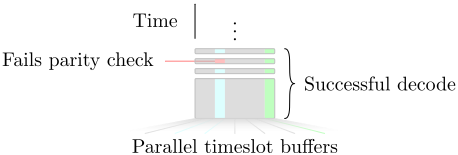
\includegraphics[width=\textwidth]{figures/burst_buffer}
  \caption{Parallel buffers used by the decoder to temporarily store
    bursts based on their frame number.}
  \label{fig:burst_buffer}
\end{figure}

In case of a wrong decision, the \gls{CRC} parity bits are checked and
an attempt is made to correct the errors, otherwise the data is
discarded. If all is well, the decoded data is passed on to the
parser.

\section{Parser}
During time synchronization, the payload of the synchronization burst
is examined after decoding and its data reveals a \gls{RFN} and a
\gls{BSIC}. The \gls{RFN} value provides information regarding the
current frame number, such that the following burst types can be
predicted. In additional to the time information, the \gls{BSIC} is
made of two identifiers, a \gls{NCC} and a \gls{BCC}. The \gls{NCC} is
an identifier unique to the vendor operating the \gls{BTS} and the
\gls{BCC} identifier specifies which training sequence, out of eight,
that is used for bursts of a normal type.

The parser extracts these properties of a synchronization burst and
updates the synchronization state machine with the knowledge of frame
synchronization. The repeating frame pattern is predictable and the
burst type following the synchronization burst is therefore known.

The real function of the parser is to visually present the properties
and content of a burst. For that reason, the parser is split over
multiple functions for each type of burst. The normal burst parser
function is the most complex, since it must determine the \gls{LAPDm}
format and from there distinguish between layer three
protocols. Common control channels are the most simple format to parse
as it uses the Bbis format, that in a general sense defines no
\gls{LAPDm} header. It has just an information field, which holds the
layer three payload. Recall the protocol discriminator values in
\cref{tab:protocol_discriminators}, in \cref{cha:design}, which define
the layer three specific payload type. The parser's implementation, as
of this writing, is limited and it only writes some of a burst's
content.
